\paragraph{QuizziPedia::Front-End::ModelViews::SignUpModelView}
	
	\label{QuizziPedia::Front-End::ModelViews::SignUpModelView}
	
	\begin{figure}[ht]
		\centering
		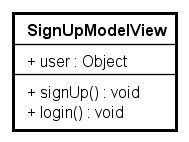
\includegraphics[scale=0.80,keepaspectratio]{UML/Classi/Front-End/QuizziPedia_Front-end_ModelView_SignUpModelView.png}
		\caption{QuizziPedia::Front-End::ModelViews::SignUpModelView}
	\end{figure} \FloatBarrier
	
	\begin{itemize}
		\item \textbf{Descrizione}: classe di tipo modelview la cui istanziazione è contenuta all'interno della variabile di ambiente \texttt{\$scope} di \textit{Angular\ped{G}}. All'interno di essa sono presenti le variabili e i metodi necessari per il \textit{Two-Way Data-Binding\ped{G}} tra la \textit{view\ped{G}} \texttt{SignUpView} e il \textit{controller\ped{G}} \texttt{SignUpController};
		\item \textbf{Utilizzo}: viene utilizzata per effettuare il \textit{Two-Way Data-Binding\ped{G}} tra la \textit{view\ped{G}} \texttt{SignUpView} e il \textit{controller\ped{G}} \texttt{SignUpController} rendendo disponibili variabili e metodi;
		\item \textbf{Relazioni con altre classi}: 
		\begin{itemize}
			\item \textbf{OUT \texttt{SignUpView}}: \textit{view\ped{G}} contenente le form dedicate alla registrazione utente. Contiene inoltre un link alla pagina di login; 
			\item \textbf{OUT \texttt{SignUpController}}: questa classe permette di gestire la registrazione di un utente al sistema.
		\end{itemize}
		\item \textbf{Attributi}: 
		\begin{itemize}
			\item \texttt{+ user: Object} \\ Campo dati contenente i seguenti attributi: \texttt{name: String}, \texttt{surname: String}, \texttt{username: String}, \texttt{email: String},\\ \texttt{password: String} e \texttt{passwordCheck: String}.
		\end{itemize}
		\item \textbf{Metodi}: 
		\begin{itemize}	
			\item \texttt{+} \texttt{signUp(user: Object): void} \\
			Metodo che richiama il metodo \texttt{signup} del service \texttt{AuthService} passandogli un oggetto di tipo \texttt{SignUpModelView}. Nel caso di buona riuscita dell'operazione viene mostrato un messaggio di successo. Con l'azione di click sul bottone presentato dal messaggio di successo è possibile effettuare il redirect alla pagina di login dell'applicazione. Nel caso in cui invece avvenga un errore, viene mostrato a video il messaggio di errore.
			\textbf{Parametri}:
			\begin{itemize}
				\item \texttt{user: Object} \\
				Parametro che rappresenta un oggetto contenente tutti i parametri per la registrazione.
			\end{itemize}
			\item \texttt{+} \texttt{logIn(): void} \\
			Metodo che gestisce l'evento click sul pulsante di login. Effettua il redirect alla pagina di login.
		\end{itemize}
	\end{itemize}
	
	